% Chapter 1 (from main tex file)
% New Trends in Research
% Author: Javier Reyes

\chapter{DAEbot Autonomous Robot}

The DAEbot project stands for Distributed Architectures Evaluation robot, a modular system that allows different approaches for distributed hardware and software architectures to be tested \cite{Wiki}.

The robot is designed and built with common hardware (evaluation boards and popular sensors-actuators), so that it can be easily replaced or tested with different devices, as well as test different software solutions or methodologies. Physically, the robot represents a layered structure, to resemble the software architecture approach that is used, which is based in the OCM software architecture.

\section{OCM architecture}

Typical mechatronic systems complexity grows exponentialy with every new technological step, which requieres a careful process of defining the right architecture for mechatronic systems. On this base concept, the goal for the DAEbot architecture is graphically represented in the figure \ref{fig:ocm}.

\begin{figure}[h]
	\centering
	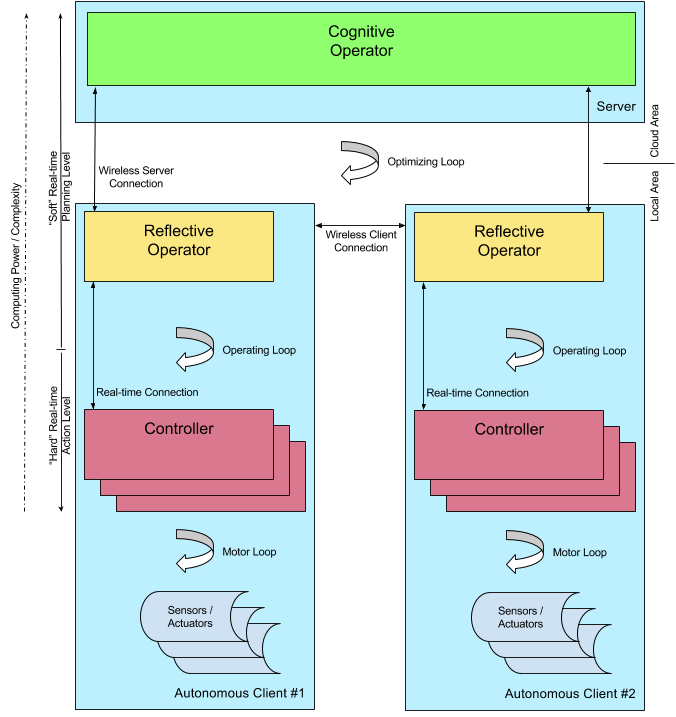
\includegraphics[width=0.6\textwidth]{ocm-architecture.png}
	\caption{OCM software architecture model.} \label{fig:ocm}
\end{figure}

The OCM structure is based on the work of the Mechatronics Laboratory Paderborn as a hierarchical structure for mechatronics systems \cite{Lueckel2001}. This structure defines three different layers that allows the clear seaparation of controllers, considering the real-time characteristics, and therefore allowing a more comprehensive development process.

\begin{description}
	\item[Controller Layer] \hfill \\ This is the lowest level layer, where the traditional controller is defined as a traditional control loop, usually based on a mathematical model. This way the controller gains flexibility in terms of the configuration parameters, and can be individually simulated and tested (XiL), allowing different operation modes which will be \textit{operated} from the next layer.
	\item[Reflective Operator] \hfill \\ On this layer, the monitoring and control is implemented, and even allow communication with other systems in a network.
	\item[Cognitive Operator] \hfill \\ For more complex systems, that need coordination/communication interactions or learning algorithms, the Cognitive layer expands the functionality.
\end{description}

The DAEbot defined structure related to the OCM architecture can be seen in figure \ref{fig:daebot}.

\begin{figure}[h]
	\centering
	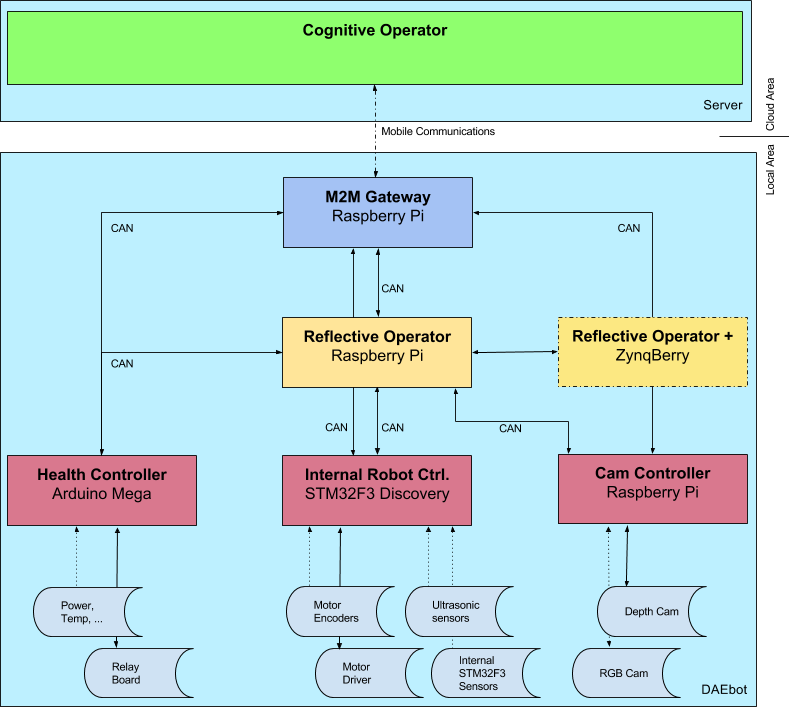
\includegraphics[width=0.6\textwidth]{dae-architecture.png}
	\caption{DAEbot architecture.} \label{fig:daebot}
\end{figure}

Given the modular architecture, the design and develoment of each of the elements in the system can be modularized and worked independently, under the guidelines of the structure.

\section{Refective Operator+ Zynqberry}

The zynqberry board, with its FPGA capababilities, is considered a second operator with the expectation of evaluating a true parallel application performance inside the OCM architecture. The communication from and to the main Reflective Operator (Raspberry Pi) and the Controllers is provided by CAN bus, with an optional link via Ethernet for high data payloads.
